\documentclass{beamer}

\usefonttheme{professionalfonts} % using non standard fonts for beamer
\usefonttheme{serif} % default family is serif

%\usepackage{hyperref}

%\usepackage{minted}

\usepackage{animate}

\usepackage{graphicx}

\def\Put(#1,#2)#3{\leavevmode\makebox(0,0){\put(#1,#2){#3}}}

\usepackage{color}

\usepackage{tikz}

\usepackage{amssymb}

\usepackage{enumerate}


\newcommand\blfootnote[1]{%

  \begingroup

  \renewcommand\thefootnote{}\footnote{#1}%

  \addtocounter{footnote}{-1}%

  \endgroup

}

\makeatletter

%%%%%%%%%%%%%%%%%%%%%%%%%%%%%% Textclass specific LaTeX commands.

 % this default might be overridden by plain title style

 \newcommand\makebeamertitle{\frame{\maketitle}}%

 % (ERT) argument for the TOC

 \AtBeginDocument{%

   \let\origtableofcontents=\tableofcontents

   \def\tableofcontents{\@ifnextchar[{\origtableofcontents}{\gobbletableofcontents}}

   \def\gobbletableofcontents#1{\origtableofcontents}

 }

%%%%%%%%%%%%%%%%%%%%%%%%%%%%%% User specified LaTeX commands.

\usetheme{Malmoe}

% or ...

\useoutertheme{infolines}

\addtobeamertemplate{headline}{}{\vskip2pt}



\setbeamercovered{transparent}

% or whatever (possibly just delete it)

\makeatother

\begin{document}
\title[DDCEL report]{A Scalable DCEL implementation}
\author[AC]{Andres Calderon}
\institute[Spring'20]{University of California, Riverside}
\makebeamertitle
\newif\iflattersubsect

% \AtBeginSection[] {
%   \begin{frame}<beamer>
%     \frametitle{Outline} 
%     \tableofcontents[currentsection]  
%   \end{frame}
%   \lattersubsectfalse
% }

\AtBeginSubsection[] {
  \begin{frame}<beamer>
    \frametitle{Outline} 
    \tableofcontents[currentsubsection]  
  \end{frame}
}

\begin{frame}{DCEL construction in CGAL...}{Incremental algorithm \footnote{\tiny{D. Halperin, “Arrangements,” in Handbook of discrete and computational geometry, USA: CRC Press, Inc., 1997, pp. 389–412.}}}

Given a collection $\mathcal{L}={l_1,...,l_i}$ of $i$ lines, we assume the DCEL $\mathcal{A}(\mathcal{L}_i)$ \\
To add next line $l_{i+1}$ do:
    \begin{enumerate}
        \item Find \textit{zone} (set of faces intersected) for $l_{i+1}$.
        \item Find point $p$ of intersection between $l_{i+1}$ and an edge of $\mathcal{A}(\mathcal{L}_i)$; split that edge.
        \item Walk along $l_{i+1}$ from $p$ to left updating $\mathcal{A}(\mathcal{L}_i)$.
        \item Walk along $l_{i+1}$ from $p$ to right completing the construction.
    \end{enumerate}
\end{frame}

\begin{frame}{DCEL construction in CGAL...}
    \centering 
    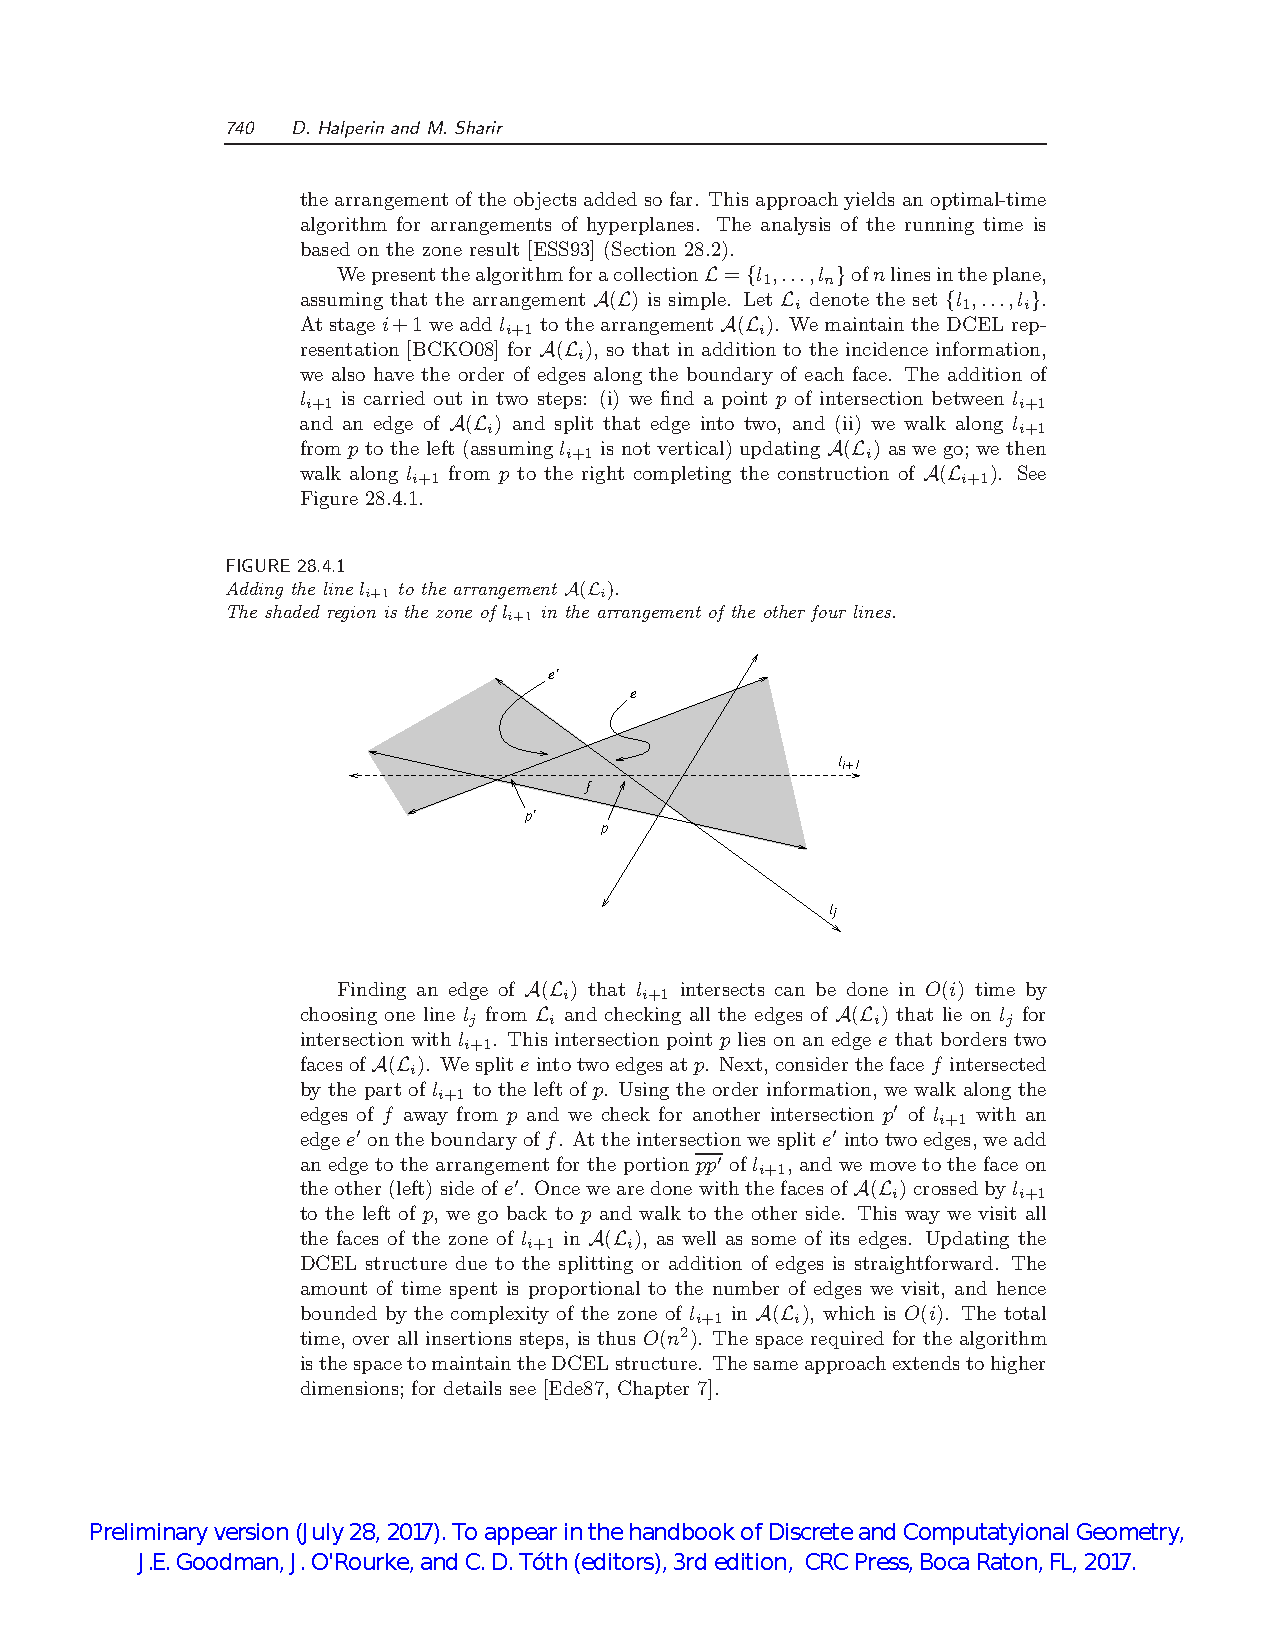
\includegraphics[trim=5.8cm 12cm 7cm 11cm, clip, width=0.9\textwidth]{figures/incremental.pdf}
\end{frame}

\begin{frame}{DCEL construction in CGAL...}
    \centering 
    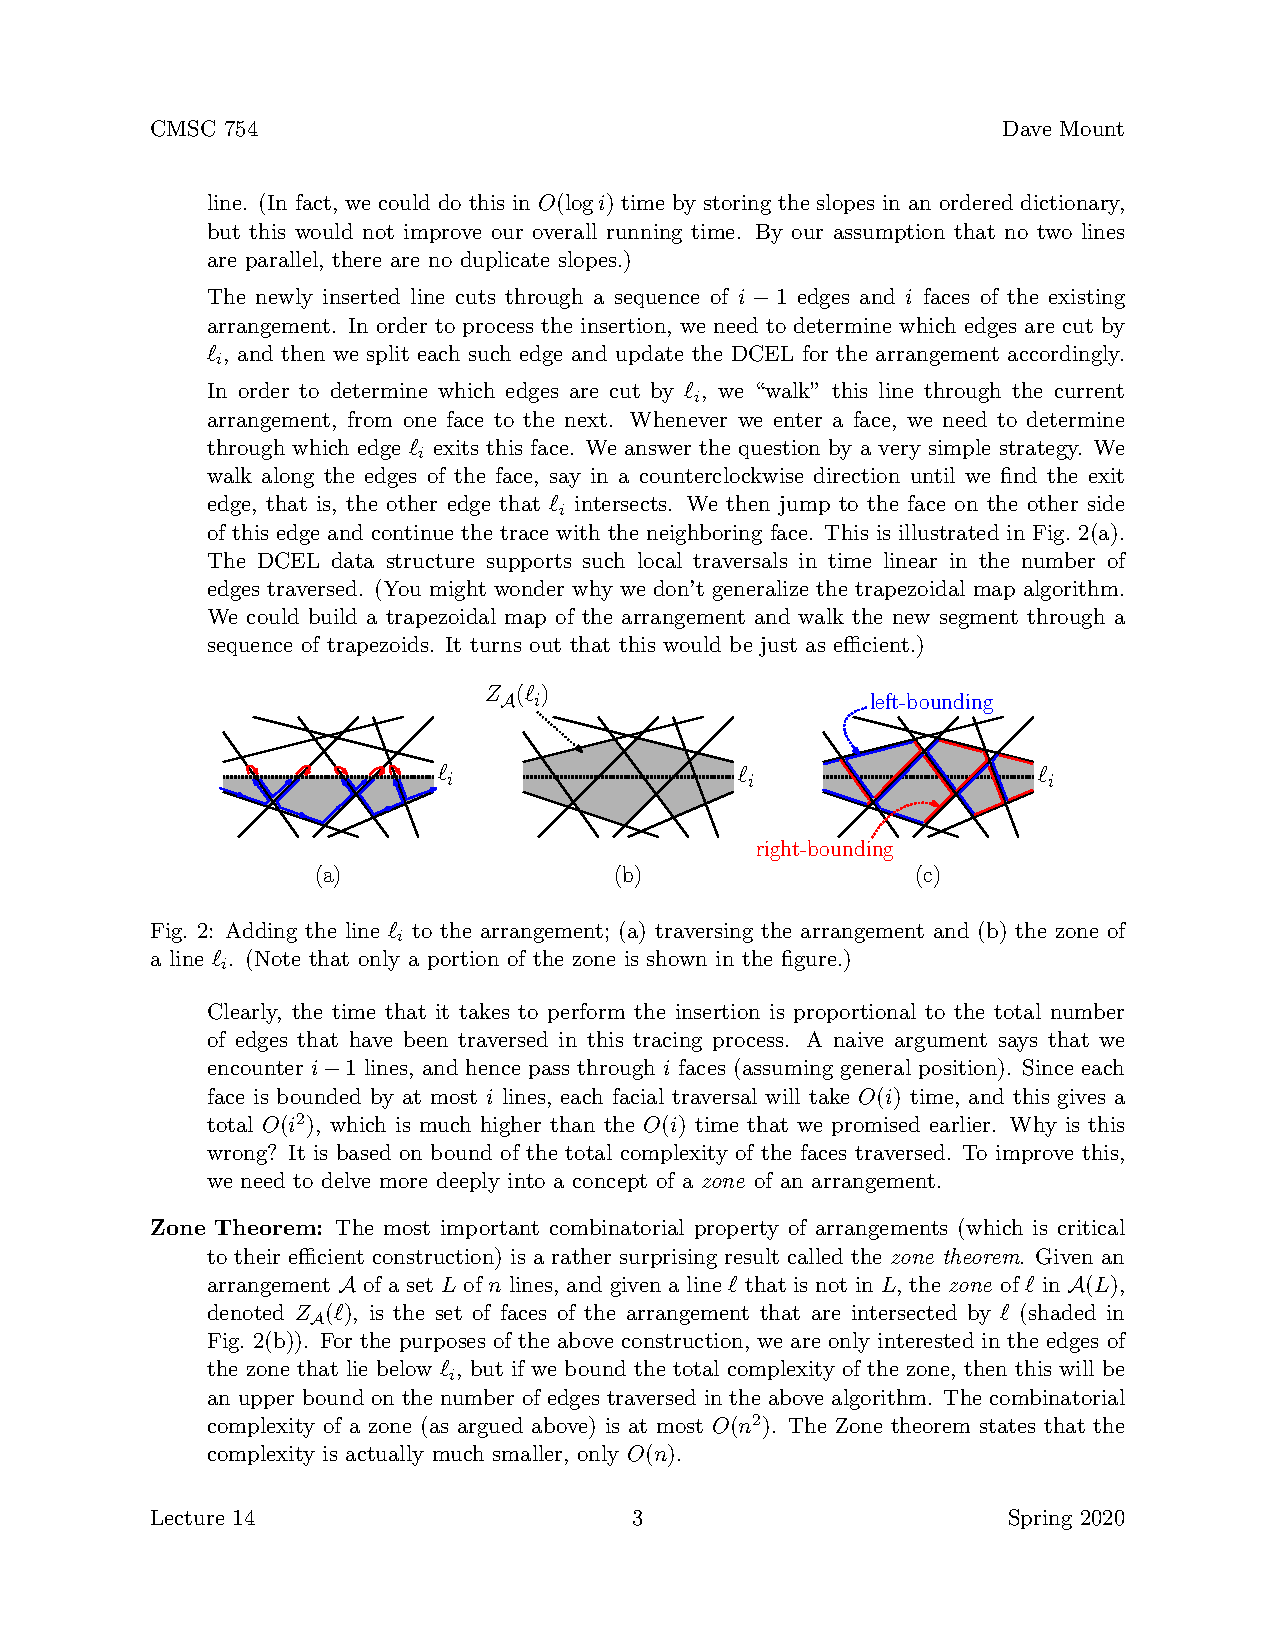
\includegraphics[trim=3cm 13.5cm 13.5cm 12cm, clip, width=0.9\textwidth]{figures/walk.pdf}
\end{frame}

\begin{frame}{DCEL merge (overlay) in CGAL...}
    \begin{itemize}
        \item I did not find a specific reference to the merge (overlay) from two DCEL in CGAL, but...
        \item Checking github repository \href{https://tinyurl.com/5cc7w7t3}{Arr\_overlay\_2.h}, it seems the strategy is to add the edges from the smaller DCEL to the bigger one using the incremental construction. 
    \end{itemize}

\end{frame}


\end{document}
